\documentclass{article}
	
\usepackage[margin=1in]{geometry}		% For setting margins
\usepackage{amsmath}				% For Math
\usepackage[]{amssymb}
\usepackage{amsmath}
\usepackage{gensymb}
\usepackage{fancyhdr}				% For fancy header/footer
\usepackage{graphicx}				% For including figure/image
\usepackage{cancel}					% To use the slash to cancel out stuff in work
\usepackage{wasysym}                % For cent symbol
\usepackage{pgfplots}
\usepackage{gnuplottex}

\pgfplotsset{width=7cm,compat=1.9}
\usepgfplotslibrary{fillbetween}

% We will externalize the figures
% \usepgfplotslibrary{external}
% \tikzexternalize

%%%%%%%%%%%%%%%%%%%%%%
% Set up fancy header/footer
\pagestyle{fancy}
\fancyhead[RO,R]{{\textbf{Andry Paez}}}
\fancyhead[LO,L]{\textbf{Ch.14}}
\fancyhead[CO,C]{\textbf{Problem Set 1}}
% \fancyhead[RO,R]{\today}
\fancyfoot[LO,L]{}
\fancyfoot[CO,C]{\thepage}
\fancyfoot[RO,R]{}
\renewcommand{\headrulewidth}{0.4pt}
\renewcommand{\footrulewidth}{0.4pt}
%%%%%%%%%%%%%%%%%%%%%%

\newcommand{\hmwkTitle}{Ch 14 - Problem Set 1}
% \newcommand{\hmwkDueDate}{February 12, 2014}
\newcommand{\hmwkClass}{Calculus 3}
% \newcommand{\hmwkClassTime}{}
% \newcommand{\hmwkClassInstructor}{Professor Isaac Newton}
\newcommand{\hmwkAuthorName}{\textbf{Andry Paez}}

% math commands
\newcommand{\ihat}{\;\hat{\textbf{\i}}}
\newcommand{\jhat}{\;\hat{\textbf{\j}}}
\newcommand{\khat}{\;\hat{\textbf{k}}}
\newcommand{\rvec}{\vec{r}(t)}
\newcommand{\drvec}{\vec{r}\;'(t)}
\newcommand\vv[1]{\langle #1 \rangle}
\newcommand\vc[2]{\vec{#1}(#2)}
\newcommand\vcd[2]{\vec{#1}\;'(#2)}
\newcommand\vcdd[2]{\vec{#1}\;''(#2)}
\newcommand\vcddd[2]{\vec{#1}\;'''(#2)}
\newcommand\mgv[1]{\|#1\|}
\newcommand\mgvv[2]{\sqrt{\left(#1\right)^2 + \left(#2\right)^2}}
\newcommand\mgvvv[3]{\sqrt{\left(#1\right)^2 + \left(#2\right)^2 + \left(#3\right)^2}}
\newcommand\rr{\quad\Rightarrow\quad}
\newcommand{\limit}[4]{\lim_{(#1, #2) \to (#3, #4)}}
\newcommand{\such}{\; | \;}
%
% Title Page
%
\title{
    \vspace{3in}
    \textmd{\textbf{\hmwkTitle}}\\
    \vspace{0.5in}
    \textmd{\textbf{\hmwkClass}}\\
    % \normalsize\vspace{0.1in}\small{Due\ on\ \hmwkDueDate\ at 3:10pm}\\
    % \vspace{0.1in}\large{\textit{\hmwkClassInstructor\ \hmwkClassTime}}
    \vspace{4in}
}

\author{\hmwkAuthorName}
\date{}

\begin{document}
\maketitle

% New blank page for printers that print on both sides of paper
\clearpage\shipout\null

\begin{center}
    \section*{\underline{Section 1: Functions of Several Variables}}
\end{center}

\subsection*{3. Let $g(x,y) = x^2\ln (x+y)$ \\ (\textit a) Evaluate $g(3, 1)$. \\ (\textit b) Find and sketch the domain of $g$. \\ (\textit c) Find the range of $g$.}
\centerline{\textbf{Solution}}
\begin{align*}
    \intertext{\textit a) 9\ln 4}
    \intertext{\textit b) $D:\{(x,y) \such y > -x\}$}
    % graph and shade region of domain
    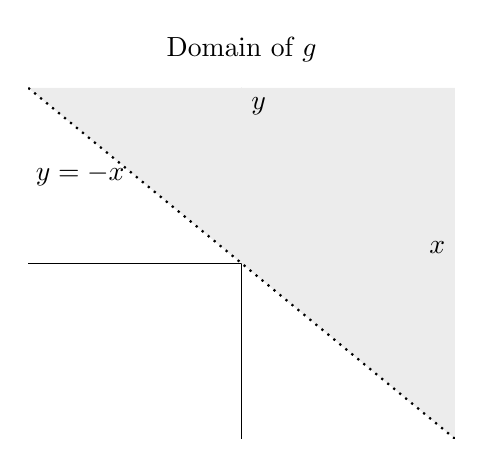
\begin{tikzpicture}
        \begin{axis} [
            title={Domain of $g$},
            axis lines=middle,
            xlabel=$x$,
            ylabel=$y$,
            ymin=-5, ymax=5,
            ticks=none,
        ]
        \addplot [
            name path=line,
            domain=-5:5,
            dotted,
            thick,
        ]
        {-x} node [left, pos=0.25] {$y=-x$};];  
        \addplot[draw=none, name path=axis] {5};
        \addplot [fill=gray!15] fill between[of=line and axis];
        \end{axis}
    \end{tikzpicture}
    \intertext{\textit c) $\mathbb R$}
\end{align*}
\subsection*{7 - 15 (odd)}

Find and sketch the domain of the function.

\subsubsection*{7. $f(x,y)=\sqrt{x-2} + \sqrt{y-1}$}
\centerline{\textbf{Solution}}
\begin{align*}
    \intertext{$D:\{(x,y)\such x\geq 2, y\geq 1\}$}
    \begin{tikzpicture}
        % Define the axis
        \draw[->] (-1,0) -- (5,0) node[right] {$x$};
        \draw[->] (0,-1) -- (0,5) node[above] {$y$};
        % Draw the lines 
        \draw (2, 5) -- (2, -1)
        \draw (-1, 1) -- (5, 1) 
        % Shade the region x >= 2 and y >= 1
        \fill[gray!15] (2,1) rectangle (5,5);
    \end{tikzpicture}
\end{align*}
\subsubsection*{9. $q(x,y)=\sqrt x + \sqrt{4- 4x^2 - y^2}$}
\centerline{\textbf{Solution}}
\begin{align*}
    \intertext{$D:\{(x,y)\such x^2+\frac 1 4 y^2\leq 1, x\geq 0\}$}
    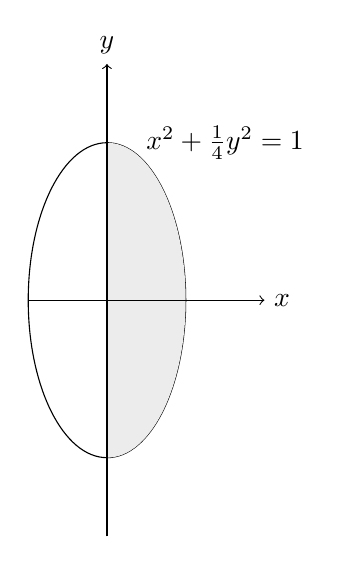
\begin{tikzpicture}
        % Draw the  ellipse 
        \draw (0, 0) ellipse (1 and 2); 
        \node at (1.5, 2) {$x^2 + \frac 1 4 y^2 = 1$};
        % Define a custom clip path to fit the inside of the ellipse
        \begin{scope}
            \clip (0,-2) -- (2,-2) -- (2,0) -- (2,2) -- (0,2) -- cycle;
            % Shade the region
            \fill[gray!15] (0,0) ellipse (1 and 2);
        \end{scope}
        % Define the axis
        \draw[->] (-1,0) -- (2,0) node[right] {$x$};
        \draw[->] (0,-3) -- (0,3) node[above] {$y$};
    \end{tikzpicture}
\end{align*}
\subsubsection*{11. $g(x,y) = \displaystyle\frac{x - y}{x + y}$}
\centerline{\textbf{Solution}}
\begin{align*}
    \intertext{$D:\{(x,y)\such y\neq -x\}$}
    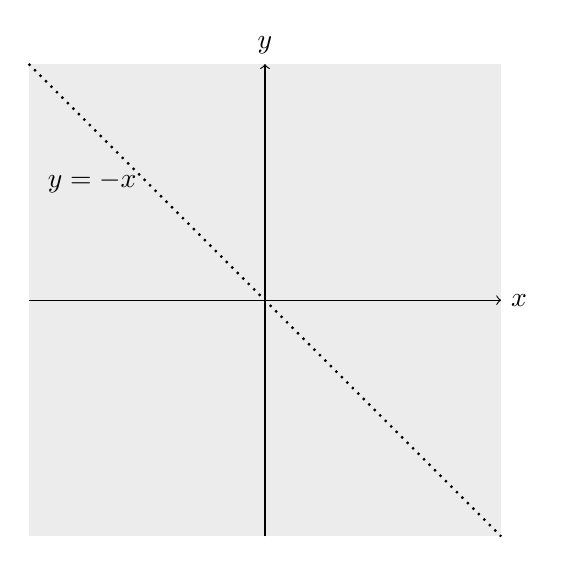
\begin{tikzpicture}
        % Shade the region y != -x
        \fill[gray!15] (-3,-3) -- (-3,3) -- (3,3) -- (3,-3) -- cycle;
        % Draw the lines 
        \draw[dotted, thick] (-3, 3) -- (3,-3) node [left, pos=0.25] {$y=-x$};
        % Define the axis
        \draw[->] (-3,0) -- (3,0) node[right] {$x$};
        \draw[->] (0,-3) -- (0,3) node[above] {$y$};
    \end{tikzpicture}
\end{align*}
\subsubsection*{13. $p(x,y) = \displaystyle\frac{\sqrt{xy}}{x+1}$}
\centerline{\textbf{Solution}}
\begin{align*}
    \intertext{$D:\{(x,y)\such x\neq 0, xy\geq 0\}$}
    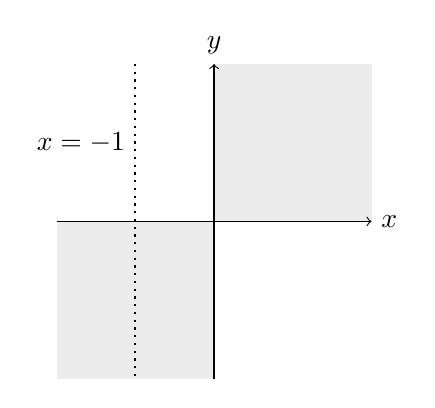
\begin{tikzpicture}
        % Shade the region xy >= 0
        \fill [gray!15] (0,0) -- (0,2) -- (2,2) -- (2,0) -- cycle;
        \fill [gray!15] (0,0) -- (0,-2) -- (-2,-2) -- (-2,0) -- cycle;
        % Draw the line x != -1
        \draw[dotted, thick] (-1,2) -- (-1,-2) node [left, pos=0.25] {$x=-1$};
        % Define the axis
        \draw[->] (-2,0) -- (2,0) node[right] {$x$};
        \draw[->] (0,-2) -- (0,2) node[above] {$y$};
    \end{tikzpicture}
\end{align*}
\subsubsection*{15. $f(x,y,z) = \sqrt{4 - x^2} + \sqrt{9 - y^2} + \sqrt{1 - z^2}$}
\centerline{\textbf{Solution}}
\subsection*{17. A model for the surface area of a human body is given by the function \\
    \begin{align*} S = f(w, h) = 0.1091w^{0.425}h^{0.725} \end{align*} \\
    where $w$ is the weight (in pounds), $h$ is the height (in inches), and $S$ is measured in square feet. \\
    (\textit a) Find $f(160, 70)$ and interpret it. \\
    (\textit b) What is your own surface area?
$}
\centerline{\textbf{Solution}}
\subsection*{23 - 31 (odd)}
Sketch the graph of the function
\subsubsection*{23. $f(x,y) = y$}
\centerline{\textbf{Solution}}
\subsubsection*{25. $f(x,y) = 10 - 4x -5y$}
\centerline{\textbf{Solution}}
\subsubsection*{27. $f(x,y) = \sin x$}
\centerline{\textbf{Solution}}
\subsubsection*{29. $f(x,y) = x^2 + 4y^2 + 1$}
\centerline{\textbf{Solution}}
\subsubsection*{31. $f(x,y) = \sqrt{4 - 4x^2 - y^2}$}
\centerline{\textbf{Solution}}
% Needs graphs or screenshot and insert as figure
\subsection*{32. Match the function with its graph (labeled I–VI). Give reasons for your choices. \\
    (\textit a) $f(x,y) = \displaystyle\frac 1 {1 + x^2 + y^2} \qquad (\textit b)\; f(x,y) = \frac 1 {1 + x^2 y^2}$ \\\\
    (\textit c) $f(x,y) = \ln (x^2 + y^2) \qquad \;(\textit d)\; f(x,y) = \cos \sqrt{x^2 + y^2}$ \\\\
    (\textit e) $f(x,y) = |xy| \qquad \qquad \quad (\textit f)\; f(x,y) = \cos (xy)$\\
}
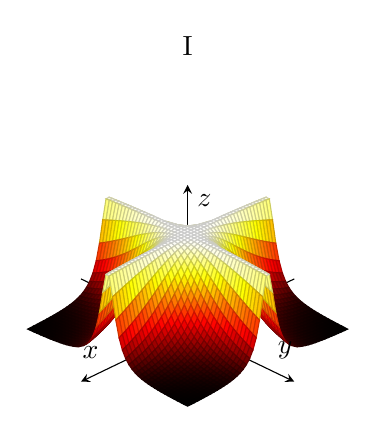
\begin{tikzpicture}
    \begin{axis}[
        title={I},
        axis lines=middle,
        xlabel=$x$,
        ylabel=$y$,
        zlabel=$z$,
        xmin=-4, xmax=4,
        ymin=-4, ymax=4,
        zmin=0, zmax=1.5,
        view={135}{45},
        ticks = none,
        colormap/hot2,
        ]
        \addplot3[
            surf,
            samples = 50,
            domain=-3:3,
        ] {1/(1+ x^2 * y^2)};
    \end{axis} 
\end{tikzpicture}
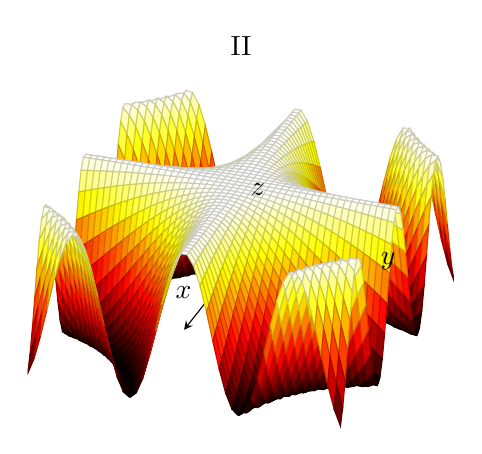
\begin{tikzpicture}
    \begin{axis}[
        title={II},
        axis lines=middle,
        xlabel=$x$,
        ylabel=$y$,
        zlabel=$z$,
        % xmin= -5, xmax= 5,
        % ymin= -5, ymax= 5,
        % zmin= 0, zmax= 5,
        view={110}{45},
        ticks = none,
        colormap/hot2,
        ]
        \addplot3[
            surf,
            samples = 50,
            domain= -3 : 3,
            domain y = -3 : 3,
        ] {cos(deg(x*y))};
    \end{axis} 
\end{tikzpicture}
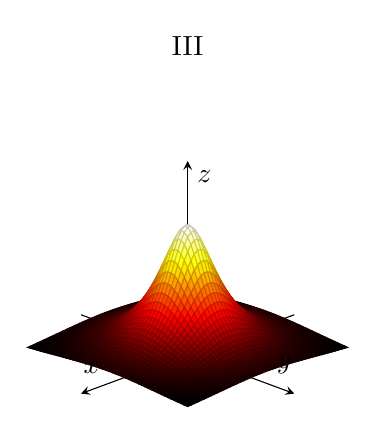
\begin{tikzpicture}
    \begin{axis}[
        title={III},
        axis lines=middle,
        xlabel=$x$,
        ylabel=$y$,
        zlabel=$z$,
        xmin=-4, xmax=4,
        ymin=-4, ymax=4,
        zmin=0, zmax=1.5,
        view={135}{30},
        ticks = none,
        colormap/hot2,
        ]
        \addplot3[
            surf,
            samples = 50,
            domain=-3:3,
        ] {1/(1+x^2+y^2)};
    \end{axis} 
\end{tikzpicture}
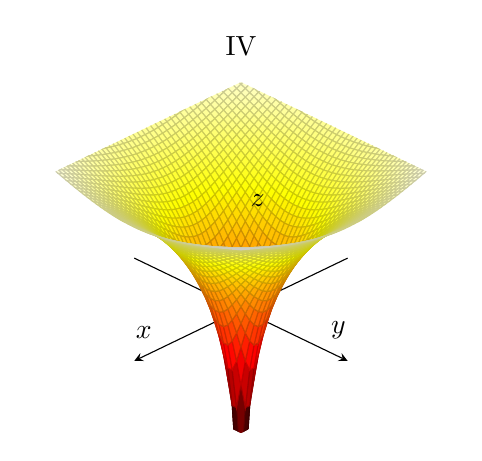
\begin{tikzpicture}
    \begin{axis}[
        title={IV},
        axis lines=middle,
        xlabel=$x$,
        ylabel=$y$,
        zlabel=$z$,
        xmin=-5, xmax=5,
        ymin=-5, ymax=5,
        zmin=-0.5, zmax=3,
        view={135}{45},
        ticks = none,
        colormap/hot2,
        ]
        \addplot3[
            surf,
            samples = 50,
            domain=-5:5,
        ] {ln(x^2 + y^2)};
    \end{axis} 
\end{tikzpicture}
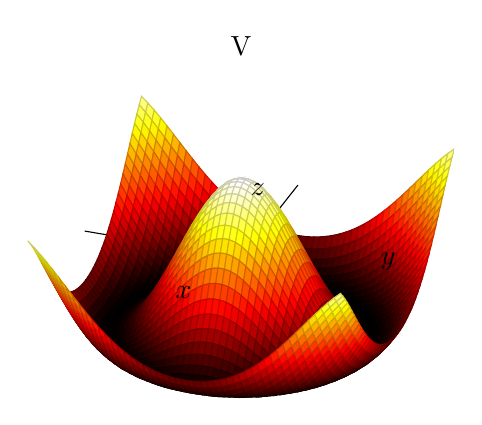
\begin{tikzpicture}
    \begin{axis}[
        title={V},
        axis lines=middle,
        xlabel=$x$,
        ylabel=$y$,
        zlabel=$z$,
        % xmin=-5, xmax=5,
        % ymin=-5, ymax=5,
        % zmin=0, zmax=4,
        view={110}{45},
        ticks = none,
        colormap/hot2
        ]
        \addplot3[
            surf,
            samples = 50,
            domain=-4:4,
        ] {cos(deg(sqrt(x^2 + y^2)))};
    \end{axis} 
\end{tikzpicture}
\begin{tikzpicture}
    \begin{axis}[
        title={VI},
        axis lines=middle,
        xlabel=$x$,
        ylabel=$y$,
        zlabel=$z$,
        xmin= -5, xmax= 5,
        ymin= -5, ymax= 5,
        zmin= 0, zmax= 20,
        view={110}{45},
        ticks = none,
        colormap/hot2,
        ]
        \addplot3[
            surf,
            samples = 50,
            domain= -5 : 5,
            domain z = 0 : 20,
        ] {abs(x*y)};
    \end{axis} 
\end{tikzpicture}
\centerline{\textbf{Solution}}
% I think this one needs a figure instead, the problem doesn't give a function 
\subsection*{33. A contour map for a function $f$ is shown. Use it to estimate the values of $f(-3, 3)$ and $f(3, -2)$. What can you say about the shape of the graph?}
\centerline{\textbf{Solution}}
\subsection*{45, 47 \& 51}
Draw a contour map of the function showing several level curves.
\subsubsection*{45. $f(x,y) = x^2 + y^2$}
\centerline{\textbf{Solution}}
\subsubsection*{47. $f(x,y) = x^2 + y^2$}
\centerline{\textbf{Solution}}
\subsubsection*{51. $f(x,y) = x^2 + y^2$}
\centerline{\textbf{Solution}}
\subsection*{53. Sketch both a contour map and a graph of the given function and compare them. \\ \begin{align*} f(x,y) = x^2 + 9y^2 \end{align*}}
\centerline{\textbf{Solution}}
% Need graphs for this one too
\subsection*{61 - 66} 
Match the function (\textit a) with its graph (labeled A–F below) and (\textit b) with its contour map (labeled I–VI). Give reasons for your choices.

\begin{figure}[h] %h = here, t = top, b = bottom, p = page of figures
    \begin{center}
        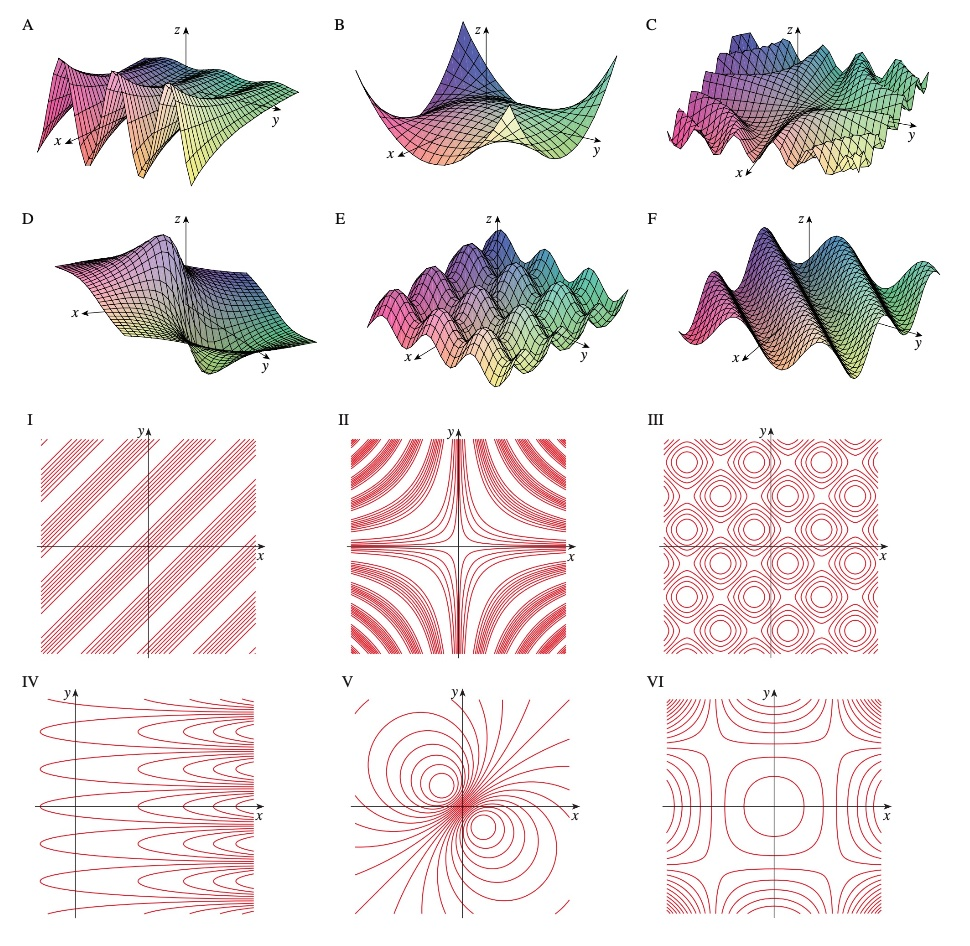
\includegraphics[width=0.95\textwidth]{figures/61-66.jpg}
    \end{center}
\end{figure}

\end{tikzpicture}
\subsubsection*{61. $z = \sin (xy)$}
\centerline{\textbf{Solution}}
\subsubsection*{62. $z = e^x \cos y$}
\centerline{\textbf{Solution}}
\subsubsection*{63. $z = \sin (x-y)$}
\centerline{\textbf{Solution}}
\subsubsection*{64. $z = \sin x - \sin y$}
\centerline{\textbf{Solution}}
\subsubsection*{65. $z = (1-x^2)(1-y^2)$}
\centerline{\textbf{Solution}}
\subsubsection*{66. $z = \displaystyle\frac{x-y}{1+ x^2+ y^2}$}
\centerline{\textbf{Solution}}
\subsection*{67. Describe the level surfaces of the function. \\ \begin{align*} f(x, y, z) = 2y - z + 1 \end{align*}}
\begin{center}
    \section*{\underline{Section 2: Limits and Continuity}}
\end{center}
\subsection*{5 - 11 (odd)}
Find the limit
\subsubsection*{5. $\lim_{(x,y) \to (3,2)} (x^2 y^3 - 4y^2)$}
\centerline{\textbf{Solution}}
\subsubsection*{7. $\limit x y {-3} 1 \displaystyle\frac{x^2 y - xy^3}{x - y - 2}$} 
\centerline{\textbf{Solution}}
\subsubsection*{9. $\limit x y \pi {\pi/2} y \sin (x - y)$}
\centerline{\textbf{Solution}}
\subsubsection*{11. $\limit x y 1 1 \left(\displaystyle\frac{x^2 y^3 - x^3 y^2}{x^2 - y^2}\right) }
\centerline{\textbf{Solution}}
\subsection*{13 - 17 (odd)}
Show that the limit does not exist
\subsubsection*{13. \limit x y 0 0 \displaystyle\frac {y^2}{x^2 + y^2}}
\centerline{\textbf{Solution}}
\subsubsection*{15. \limit x y 0 0 \displaystyle\frac {(x+y)^2}{x^2 + y^2}}
\centerline{\textbf{Solution}}
\subsubsection*{17. \limit x y 0 0 \displaystyle\frac{y^2 \sin^2 x}{x^4 + y^4}}
\centerline{\textbf{Solution}}
\subsection*{19 - 25 (odd)}
Find the limit, if it exists, or show that the limit does not exist.
\subsubsection*{19. \limit x y {-1} {-2} (x^2y-xy^2+3)^3}
\centerline{\textbf{Solution}}
\subsubsection*{21. \limit x y 2 3 \displaystyle\frac{3x - 2y}{4x^2 - y^2}}
\centerline{\textbf{Solution}}
\subsubsection*{23. \limit x y 0 0 \displaystyle\frac{xy^2\cos y}{x^2 + y^4}}
\centerline{\textbf{Solution}}
\subsubsection*{25. \limit x y 0 0 \displaystyle\frac{x^2+y^2}{\sqrt{x^2+y^2+1}-1}}
\centerline{\textbf{Solution}}
\subsection*{31 \& 33}
Use the Squeeze Theorem to find the limit.
\subsubsection*{31. \limit x y 0 0 xy\sin \displaystyle\frac 1 {x^2+y^2}}
\centerline{\textbf{Solution}}
\subsubsection*{33. \limit x y 0 0 \displaystyle\frac{xy^4}{x^4 + y^4}}
\centerline{\textbf{Solution}}
\subsection*{41, 43 \& 45}
Determine the set of points at which the function is continuous.
\subsubsection*{41. $F(x,y) = \displaystyle\frac{xy}{1+e^{x-y}}$}
\centerline{\textbf{Solution}}
\subsubsection*{43. $F(x,y) = \displaystyle\frac{1+x^2+y^2}{1-x^2-y^2}$}
\centerline{\textbf{Solution}}
\subsubsection*{45. $G(x,y) = \sqrt x + \sqrt{1 - x^2 - y^2}$}
\centerline{\textbf{Solution}}
\end{document}
